\icode{N25Z-MM-SI-L3-261011-002}
\nceeID[3]{2025浙江1月}{8}
如图所示，光滑水平地面上放置完全相同的两长板\(A\)和\(B\)，滑块\(C\)（可视为质点）置于\(B\)的右端，三者质量均为\qty{1}{kg}。\(A\)以\qty{4}{m/s}的速度向右运动，\(B\)和\(C\)一起以\qty{2}{m/s}的速度向左运动，\(A\)和\(B\)发生碰撞后粘在一起不再分开。已知\(A\)和\(B\)的长度均为\qty{0.75}{m}，\(C\)与\(A\)、\(B\)间动摩擦因数均为0.5，则\paren[]

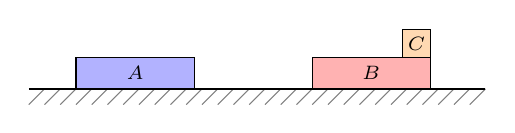
\begin{tikzpicture}[font=\scriptsize]
	\draw[fill=blue!30] (-.5,0) rectangle(1,.4)node[pos=.5]{\(A\)};
	\draw[fill=red!30] (2.5,0) rectangle(4,.4)node[midway]{\(B\)};
	\draw[fill=orange!30] (3.65,.4) rectangle(4,.75)node[pos=.5]{\(C\)};
	\foreach \x in {-1.1,-.9,...,4.6}
		\draw[gray] (\x,-.2)--++(.2,.2);
	\draw[thick] (-1.1,0)--(4.7,0);
\end{tikzpicture}
\begin{choices}
	\item 碰撞瞬间\(C\)相对地面静止
	\item 碰撞后到三者相对静止，经历的时间为\qty{0.2}{s}
	\item 碰撞后到三者相对静止，摩擦产生的热量为\qty{12}{J}
	\item 碰撞后到三者相对静止，\(C\)相对长板滑动的距离为\qty{0.6}{m}
\end{choices}
\begin{answer}
	D\qquad 提示：三者最终静止
\end{answer}